\documentclass[journal]{IEEEtran}

\usepackage[T1]{fontenc}
\usepackage{amsmath,amssymb}
\usepackage{graphicx}
\usepackage{booktabs}
\usepackage{multirow}
\usepackage{siunitx}
\usepackage{tikz}
\usepackage{pgfplots}
\pgfplotsset{compat=1.17}
\usetikzlibrary{shapes.geometric,arrows.meta,positioning,fit}
\usepackage{algorithm}
\usepackage{algpseudocode}
\usepackage{url}
\usepackage{xcolor}

\sisetup{detect-weight=true, detect-family=true}

\begin{document}

\title{From Feasibility to a Measured Timetable: A Taasika-to-UniTime Pipeline at a Computer Engineering Department}

\author{Mihir~Shah, Riya~Kulkarni, Ved~Mundhada, and Akshay~Sathaye\\
\textit{Department of Computer Engineering, COEP Technological University, Pune, India}\\
\textit{Guide: Abhijit A.\ M.}}

\markboth{Preprint, COEP Technological University}{Shah \MakeLowercase{\textit{et al.}}: Taasika-to-UniTime Pipeline}

\maketitle

\begin{abstract}
University course timetabling is an NP-hard assignment problem in which classes, instructors, student cohorts, and rooms must be placed in a weekly grid under hard and soft constraints. An earlier feasibility study showed that UniTime, an open-source scheduler built on the CPSolver library, could express every scheduling rule of a Computer Engineering department without relaxation, but it did not produce a timetable from institutional data. This paper reports the phase that closed that gap. A reproducible pipeline converted a snapshot of the department’s scheduling database into the sixteen ordered XML documents required by UniTime’s Data Exchange interface, covering one academic session, 56 course offerings comprising 291 classes, 115 instructors, 42 rooms, and 1,130 simulated students with 9,148 section enrolments. An independent evaluator, cross-validated against a second Java-based implementation to exact agreement, re-derived every reported quantity from the input files rather than from the solver’s own counters. It showed that several earlier runs reporting zero student conflicts were artifacts of silent re-sectioning, an already-solved instance, or an empty student population. With enrollments pinned, the final solution placed 290 of 291 classes with no instructor or room double-booking and achieved a hard feasibility score of 98.85 out of 100. Forty of the 1,130 students had a genuine timetable clash, all first-year students in one laboratory-lecture pairing. A reinforcement-learning layer that selected among eight CPSolver neighbourhood operators was also implemented. Its pre-registered control experiment showed that raising the solver’s student-conflict weight alone cleared the improvement threshold set for the learned policy; therefore, no claim is made that learning outperforms a correctly tuned baseline on this instance.
\end{abstract}

\begin{IEEEkeywords}
course timetabling, constraint programming, UniTime, CPSolver, iterative forward search, student conflicts, reinforcement learning.
\end{IEEEkeywords}

\section{Introduction and Problem Statement}
\label{sec:intro}

A university timetable is, at bottom, a very large pile of classes that must each land somewhere in a weekly grid. Every class brings its own room, its own instructor and its own duration, and a long list of hard and soft constraints decides which landings count as acceptable. The problem is NP-hard. No polynomial-time exact algorithm is known, so working systems lean on heuristic or metaheuristic search~\cite{schaerf1999survey}.

The Department of Computer Engineering at COEP Technological University is a stubborn instance. It runs four undergraduate years and a postgraduate programme, each cut into lecture divisions and then into laboratory batches. On top of that sit departmental electives, minor-degree courses taught by other departments, open electives, and reserved first-year blocks. Laboratory sections of a course run in parallel, while its lectures run jointly. The natural scheduling unit is therefore neither the course nor the student but the section, and it is the relationships between sections that make a timetable usable or useless.

An earlier feasibility study evaluates UniTime, an open-source, web-based scheduling system built on the CPSolver constraint library. It deploys the system locally, enters representative test data, and maps the institution's rules onto UniTime's constraint model. Its conclusion is that every identified rule is expressible, with no relaxation and no external post-processing. But that is a claim about a platform, not about a timetable. No institutional data is loaded at that stage, no solution comes from real course structure, and nothing measures solution quality. The data pipeline, the student records and the evaluation framework all remain promises.

Closing that gap matters beyond one department. A model that can \emph{express} every rule says nothing about three further questions. Can a real snapshot of a real scheduling database become solver input without manual re-entry? Is the resulting schedule good by any measure the institution cares about? Can that measure be trusted at all? Each has a less obvious answer than expected, and the third takes up most of this paper. A scheduler that quietly reports a better number than the timetable deserves is arguably worse than one that honestly reports a mediocre one, because the first invites a decision-maker to stop looking for a problem that is still there.

The present phase, run under the project name \emph{taasika-v3}, closes the gap. It contributes the following.
\begin{enumerate}
\item A reproducible pipeline reads a snapshot of the department's existing \emph{Taasika} scheduling database and emits the sixteen ordered XML documents that UniTime's Data Exchange interface consumes.
\item Institution-specific rules are encoded as generated preference data rather than entered by hand. These are the minor-degree and open-elective time blocks, the division and batch structure, and dynamic lunch breaks for students and instructors.
\item An independent evaluation framework scores any exported timetable against the same input data. A solver's own quality report cannot audit the solver, so the check has to live outside it.
\item An honest account of solution quality. Several configurations report zero student conflicts, and each turns out to be an artefact rather than an improvement. A final, pinned-enrolment solution is reported in their place.
\item A reinforcement-learning layer that chooses among stock CPSolver neighbourhood operators. Its pre-registered control experiment answers its own research question in the negative.
\end{enumerate}

\subsection{Related work}
Automated timetabling has a long history as a constraint-satisfaction and optimisation problem. Surveys of the field keep returning to constraint programming and local search as the dominant methodologies for university course timetabling, largely because both can mix mandatory and preferential requirements in a single model~\cite{schaerf1999survey}. UniTime and its embedded solver, CPSolver~\cite{cpsolver}, are one mature example. CPSolver combines Iterative Forward Search with Conflict-based Statistics~\cite{muller2004constraint} and does well in international timetabling competitions~\cite{muller2009itc,muller2025itc}. The minimal-perturbation formulation that grows up beside it addresses a very practical need: a re-solved timetable should disturb as few existing placements as possible~\cite{muller2007minimal}. Murray, M\"uller and Rudov\'a set out how an institution's offerings, subparts and sections map onto the model~\cite{murray2007modeling}. Later accounts describe the same system in daily use~\cite{rudova2011complex}, including elective courses and multiple sections~\cite{muller2016curriculum}. Soft requirements enter as weighted criteria, not as extra hard constraints~\cite{rudova2003soft}.

The published literature says much less about two things. One is the \emph{operational} route from an institution's own legacy database into such a system. The other, and the more worrying, is how easily a scheduler's reported conflict count can be made to look better than the timetable really is once students may move between sections. This second gap, not any weakness in the constraint model, is what the paper is about. The feasibility phase already shows the model is adequate. What remains open is whether a working pipeline can be built on it, and whether its output can be measured honestly.

\subsection{Scheduling model}
In the CPSolver model the decision variable is a class, meaning a single lecture, laboratory or tutorial section. Its value is a placement: a start time plus the room or rooms where the class meets. Students are not variables. A student's timetable falls out of the placements chosen for the classes that student attends, and an overlap between two classes is priced through a joint-enrolment constraint between them. So the solver has only two ways to improve a student's timetable. It can move a class, or, if allowed, it can move the student into a different section. The second route is the one that later sections expose as a source of illusory improvement. Student sectioning is a problem in its own right~\cite{muller2010sectioning}, not a side effect of timetabling.

Hard constraints hold in every acceptable timetable. No room or instructor hosts two overlapping classes. A class sits only in a room whose capacity and type suit it. Every class respects its declared meeting pattern and the term's date pattern, and weekends are excluded. Soft constraints describe quality rather than legality: preferred rooms and times, balanced instructor load, limited back-to-back teaching, a protected lunch window, and, the one this paper treats as primary, the number of students whose personal timetable contains an overlap.

\subsection{The measurement problem}
\label{sec:measurement-problem}
Producing a feasible timetable is not the hard part here. Coverage, room and instructor feasibility arrive early. The hard part is that student-conflict counts cannot be trusted, because three separate mechanisms push the reported figure toward zero without helping any student.

The first is \emph{re-sectioning}. UniTime shuffles students between parallel laboratory batches until the overlaps vanish, while the placements themselves never change. The second is an \emph{empty student population}: a demand setting that loads zero students reports zero conflicts over an empty denominator. The third is a \emph{denominator mismatch}. A conflict rate computed over the students who carry enrolments in a solver export is simply not comparable to one computed over every student in the source data.

Sections~\ref{sec:evaluator} and~\ref{sec:results} therefore treat the task as two objectives, not one. First, produce a feasible timetable. Second, establish a measurement of student conflicts that none of these three mechanisms can satisfy.

\subsection{Solver mechanics}
CPSolver is a local-search framework with constraint-programming primitives, built on Iterative Forward Search (IFS)~\cite{muller2004constraint}. IFS departs from classical local search in one respect: it works over solutions that are feasible but possibly incomplete. Some classes may stay unassigned, yet every hard constraint holds for those that are assigned, so an intermediate solution always makes sense to a human scheduler. Starting from an initial timetable, each iteration picks a class and a placement, removes the assignments that hard-conflict with it, installs the new one, and remembers the best timetable seen so far.

Fig.~\ref{fig:ifs} shows the loop as it runs in this project, including the difference between proposing a move and committing it. The reinforcement-learning layer of Section~\ref{sec:rl} replaces only the \emph{Propose move} step. That step draws one assignment from the neighbourhood of the current one, the mechanism M\"uller describes in his thesis~\cite{muller2005thesis}. CPSolver exposes the neighbourhood choice through its \texttt{NeighbourSelection} extension point. The competition solver's time changes, room changes and swaps appear in~\cite{muller2009itc}, and later changes to that set in~\cite{muller2016evolution}. A great-deluge rule decides whether a proposed move is accepted~\cite{dueck1993deluge}.

IFS is further augmented with Conflict-based Statistics (CBS)~\cite{muller2004constraint}. CBS records how often each assignment has historically caused a hard conflict with another, and during value selection it penalises candidate placements accordingly. The search drifts away from historically troublesome regions. Throughout, \texttt{Basic.DisobeyHard} is \texttt{false}, so every mechanism described later inherits the guarantee that a persisting assignment never violates a hard constraint.

\begin{figure}[t]
\centering
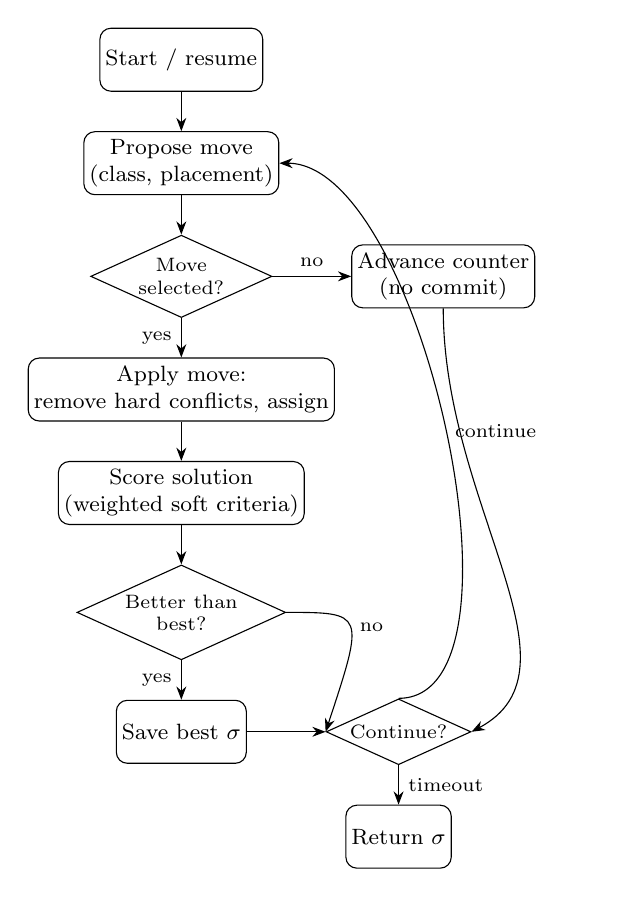
\begin{tikzpicture}[
    node distance=5mm and 6mm,
    box/.style={draw, rounded corners, align=center, minimum height=8mm, font=\footnotesize, inner sep=2pt},
    dec/.style={draw, diamond, aspect=2.2, align=center, font=\scriptsize, inner sep=1pt},
    >=Stealth
]
\node[box] (start) {Start / resume};
\node[box, below=of start] (propose) {Propose move\\(class, placement)};
\node[dec, below=of propose] (hasmove) {Move\\selected?};
\node[box, below=of hasmove] (apply) {Apply move:\\remove hard conflicts, assign};
\node[box, below=of apply] (score) {Score solution\\(weighted soft criteria)};
\node[dec, below=of score] (better) {Better than\\best?};
\node[box, below=of better] (save) {Save best $\sigma$};
\node[box, right=10mm of hasmove] (advance) {Advance counter\\(no commit)};
\node[dec, right=10mm of save] (cont) {Continue?};
\node[box, below=of cont] (ret) {Return $\sigma$};

\draw[->] (start) -- (propose);
\draw[->] (propose) -- (hasmove);
\draw[->] (hasmove) -- node[left, font=\scriptsize]{yes} (apply);
\draw[->] (hasmove) -- node[above, font=\scriptsize]{no} (advance);
\draw[->] (apply) -- (score);
\draw[->] (score) -- (better);
\draw[->] (better) -- node[left, font=\scriptsize]{yes} (save);
\draw[->] (save) -- (cont);
\draw[->] (better.east) .. controls +(10mm,0) .. node[right, font=\scriptsize]{no} (cont.west);
\draw[->] (advance.south) .. controls +(0,-25mm) and +(15mm,8mm) .. (cont.east);
\draw[->] (cont) -- node[right, font=\scriptsize]{timeout} (ret);
\draw[->] (cont.north) .. controls +(18mm,0) and +(18mm,0) .. node[right, font=\scriptsize]{continue} (propose.east);
\end{tikzpicture}
\caption{The CPSolver Iterative Forward Search loop as configured in this project. The incumbent $\sigma$ is updated only when the comparator judges the new solution better. The reinforcement-learning layer of Section~\ref{sec:rl} substitutes only the \emph{Propose move} step.}
\label{fig:ifs}
\end{figure}

UniTime models a course hierarchically. An instructional offering carries one or more configurations, each configuration holds scheduling subparts (a lecture subpart and a laboratory subpart, say), and each subpart holds the classes that actually get placed. This hierarchy lets a course with joint lectures and parallel laboratory batches live as a single offering. It also explains why the institution's division-and-batch structure maps onto UniTime without distortion.

\section{Data and Institution-Specific Constraints}
\label{sec:data}

\subsection{Source system and pipeline}
\emph{Taasika} is the scheduling database the institution already uses. A SQL dump of it holds the data as a run of numbered snapshots, each a complete picture of the departmental schedule at one moment. The pipeline parses that dump as text instead of restoring it into a database server. This is deliberate. The loader reads the dump and exposes each table as a list of records filtered to a chosen snapshot, so nothing downstream depends on a database, and the dump stays immutable input.

Fig.~\ref{fig:pipeline} traces the whole path from SQL dump to scored timetable. Eight generator modules run in dependency order and cover the session, curriculum structure, rooms, instructors, course offerings, scheduling preferences and a simulated student body. Three validators check the result, and an archive step produces the ZIP file that UniTime's Data Exchange page accepts. The sixteen documents must go in a fixed order, since each later file points at entities an earlier one creates. The time-pattern and date-pattern preferences matter most here. They have to precede the student records, or UniTime treats the classes as ``arrange hours'' and never loads them into the solver at all.

\begin{figure}[t]
\centering
\resizebox{\linewidth}{!}{%
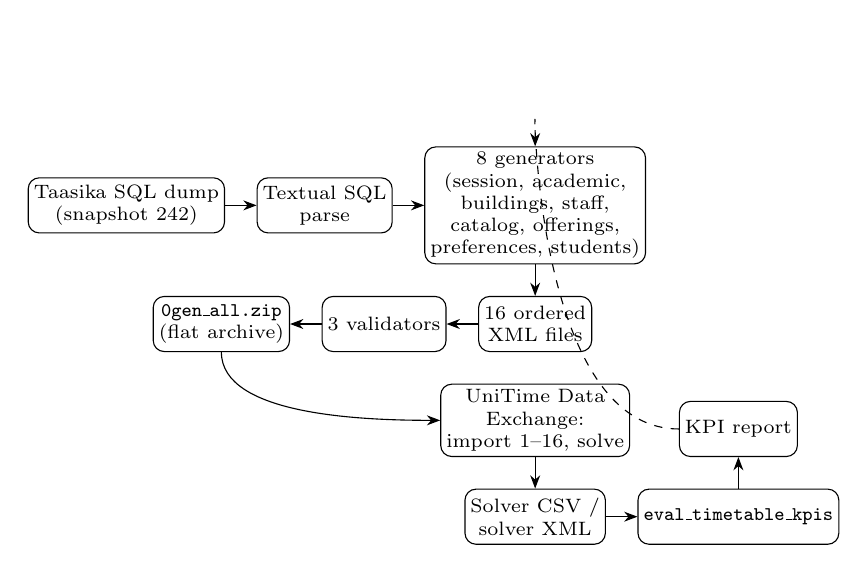
\begin{tikzpicture}[
    node distance=4mm and 4mm,
    box/.style={draw, rounded corners, align=center, font=\scriptsize, inner sep=2pt, minimum height=7mm},
    >=Stealth
]
\node[box] (sql) {Taasika SQL dump\\(snapshot 242)};
\node[box, right=of sql] (loader) {Textual SQL\\parse};
\node[box, right=of loader] (gen) {8 generators\\(session, academic,\\buildings, staff,\\catalog, offerings,\\preferences, students)};
\node[box, below=of gen] (xml) {16 ordered\\XML files};
\node[box, left=of xml] (val) {3 validators};
\node[box, left=of val] (zip) {\texttt{0gen\_all.zip}\\(flat archive)};
\node[box, below=of xml] (import) {UniTime Data\\Exchange:\\import 1--16, solve};
\node[box, below=of import] (export) {Solver CSV /\\solver XML};
\node[box, right=of export] (eval) {\texttt{eval\_timetable\_kpis}};
\node[box, above=of eval] (report) {KPI report};

\draw[->] (sql) -- (loader);
\draw[->] (loader) -- (gen);
\draw[->] (gen) -- (xml);
\draw[->] (xml) -- (val);
\draw[->] (val) -- (zip);
\draw[->] (zip.south) .. controls +(0,-8mm) and +(-10mm,0) .. (import.west);
\draw[->] (import) -- (export);
\draw[->] (export) -- (eval);
\draw[->] (eval) -- (report);
\draw[->, dashed] (report.west) .. controls +(-20mm,0) and +(0,15mm) .. (gen.north);
\end{tikzpicture}}
\caption{The taasika-v3 pipeline. Data flows from the SQL snapshot to a scored timetable; the dashed return path is the refinement loop of Section~\ref{sec:evaluator}.}
\label{fig:pipeline}
\end{figure}

\subsection{Dataset}
The working dataset, \texttt{unitime-out/0gen\_all}, carries the term attribute \texttt{Spr12} and year 2026 throughout, which gives the Data Exchange term identifier \texttt{Spr122026}. It comes from Taasika snapshot 242, named \texttt{published-v4-26jan26}. The label alone is not enough to settle this, so the snapshot is identified by cross-checking entity counts against the source database. Four of the generated documents carry a hard-coded attribute naming snapshot 240, a stale string left behind by an earlier generator version and never updated when a different snapshot is chosen. Snapshot 242 is the right one, and every figure in this paper uses it.

Table~\ref{tab:inventory} gives the inventory, recomputed directly from the generated files.

\begin{table}[t]
\centering
\caption{Inventory of \texttt{unitime-out/0gen\_all} (term Spr122026).}
\label{tab:inventory}
\footnotesize
\begin{tabular}{@{}ll@{}}
\toprule
File & Contents \\
\midrule
1sessionSetup & session, departments, subject areas, patterns \\
2academicArea & 2 areas (B.Tech, M.Tech) \\
3academicClassification & 5 year codes (FY, SY, TY, BT, MT) \\
4Major / 5Minor & 15 majors; minors modelled as majors \\
6studentGroup & 242 groups (43 classes + 199 batches) \\
7buildingRoomImport & 6 buildings, 42 rooms \\
8roomSharing & 45 sharing blocks; weekends unavailable \\
9travelTimes & 7 inter-building travel entries \\
10staff & 115 instructors \\
11courseCatalog & 158 courses \\
12courseOffering & 56 offerings, 84 subparts, 291 classes \\
13preferences & 362 preference blocks \\
14studentInfo & 1{,}130 students, 5{,}767 group refs. \\
15studentRequest & requests for 1{,}130 students \\
16studentenrollments & 9{,}148 section enrolments \\
\bottomrule
\end{tabular}
\end{table}

Table~\ref{tab:population} describes the simulated student population. Institutional MIS data is not available, so the student body is built from headcounts confirmed with the department. The simulation allocates students to lecture divisions, then to laboratory batches. It then issues a course request for every compulsory subject and one per elective group, and finally enrols each student in a concrete lecture and laboratory section. No real student data appears anywhere in the dataset. Every identifier is synthetic.

\begin{table}[t]
\centering
\caption{Simulated student population of the current dataset.}
\label{tab:population}
\footnotesize
\begin{tabular}{@{}lrrl@{}}
\toprule
Year & CSE & AI\&ML & Total / structure \\
\midrule
First year (FY) & 300 & 100 & 400, single cohort \\
Second year (SY) & 200 & 0 & 200, two lecture divisions \\
Third year (TY) & 200 & 0 & 200, two divisions \\
Final year (BT) & 200 & 0 & 200, two divisions \\
M.Tech (MT) & \multicolumn{2}{c}{130} & specialization streams \\
\midrule
Total & \multicolumn{2}{c}{} & \textbf{1{,}130}, all with enrollments \\
\bottomrule
\end{tabular}
\end{table}

\subsection{Institution-specific constraints as generated data}
The mapping from institutional rule to UniTime construct comes out of the earlier feasibility phase. It shows that a rule \emph{can} be expressed, and that is all it shows, since it schedules nothing. The job in this phase is to generate the matching preference data for every class in the dataset. The rules then reproduce themselves on each pipeline run, with no re-entry by hand after an import.

The institution reserves fixed windows in the week for course categories taught across departments. Minor-degree courses meet on Monday and Tuesday evenings, and open electives on Monday and Tuesday mornings. These are hard commitments, and they have a second half that is easy to miss. Reserving a window for one category achieves nothing unless every other course is kept out of it. A small rule engine handles both halves. It is consulted for every scheduling subpart, and the first rule whose course pattern matches, and whose exclusion pattern does not, becomes active for that subpart. Table~\ref{tab:blocks} lists the four rules in force.

\begin{table}[t]
\centering
\caption{The fixed time-block rules, in evaluation order.}
\label{tab:blocks}
\footnotesize
\begin{tabular}{@{}lllc@{}}
\toprule
Rule & Days & Window & Level \\
\midrule
MDM required & Mon, Tue & 16:30--18:30 & Required \\
OE required & Mon, Tue & 09:30--10:30 & Required \\
Non-MDM prohibited & Mon, Tue & 16:30--18:30 & Prohibited \\
SY non-OE prohibited & Mon, Tue & 09:30--10:30 & Prohibited \\
\bottomrule
\end{tabular}
\end{table}

A required rule pins one slot matching the day set and window to a matching course. A prohibited rule clears every other candidate class whose days and interval overlap the window. Rules run in the order shown, and only the first applicable one governs a given subpart, so a course that happens to match two patterns still answers to a single rule. The second-year prohibition is written course by course, not by wildcard, because only that year's core subjects share the open-elective morning.

The dataset also declares 242 student groups, one for each class and each laboratory batch, and every student joins the groups matching the classes they attend. This makes the cohort structure visible in the UniTime interface and is a prerequisite for a possible future group reservation. It does not, by itself, constrain the timetable. With student switching disabled, as Section~\ref{sec:zero-conflict} requires, a student's groups only affect a distance computation for students not yet enrolled, and the final sectioning pass never reads them. What really pins a student to a section is the enrolment file together with the three solver settings of Section~\ref{sec:zero-conflict}. The group data is informative, not load-bearing, and adding it changes no placement and no conflict count. Laboratories jointly supervised by two instructors for one batch use UniTime's native support for multiple lead instructors on a single class, the same mechanism the pipeline already uses to emit one laboratory class per batch record.

The dynamic one-hour lunch break falls between 11:30 and 15:30 and applies separately to students and to instructors. It is implemented as a solver-side criterion, not as a blocked slot in the time patterns. A universal blocked hour would remove the same window from every day for every class, whereas the institution wants only that each person has \emph{some} free hour inside the window. The criterion is soft, so the solver may violate it. Section~\ref{sec:results} reports how often it does.

\subsection{Translating a legacy schema}
Translating Taasika into UniTime also means resolving a handful of structural mismatches between the two data models. None is a scheduling rule in the sense of Table~\ref{tab:blocks}, yet each decides whether the generated data is interpretable by the solver at all.

A laboratory or tutorial subject is merged into its lecture partner whenever its short name is the lecture's short name plus a recognised suffix. A joint lecture and its parallel laboratory batches then become one offering with two scheduling subparts, not two unrelated courses. Credits follow the local engineering convention: one credit per weekly lecture hour, half a credit per laboratory hour. Unpaired subjects fall back to the lecture-only or laboratory-only half of the same formula, with a floor of one credit. Class identifiers are built to be readable and stable, made of an area code, a course number, a type and a suffix. The student-enrolment documents reference exactly these identifiers, so an unstable scheme would quietly break the dependency chain in Table~\ref{tab:inventory}.

Taasika records room names but not buildings. A heuristic on room and subject short names therefore assigns each room to one of six inferred buildings. Laboratories that are not actually usable go into a separate pool, so any use of them stays visible in the evaluation and cannot hide among normal rooms. Instructor rank is derived from each teacher's declared minimum- and maximum-hours envelope, because Taasika has no rank field.

Last, and most important for Section~\ref{sec:evaluator}, no class carries an explicit time in the generated data. The existing Taasika timetable rows are deliberately not imported as time preferences. The aim is for UniTime to solve the timetable from scratch, not to reproduce the hand-built one. Room associations from Taasika are likewise emitted as preferences, not pre-assignments, so the solver is free to place each class in any suitable room.

\subsection{Identifying the source snapshot}
The Taasika dump stores many numbered snapshots, and the generated XML's own provenance string proves unreliable. Which snapshot produced the working dataset therefore has to be settled by evidence, not by a label. Table~\ref{tab:snapshot} compares three candidates against the final dataset on three counts the generators carry over almost unchanged from the source: student groups (one per class plus one per laboratory batch), teachers, and rooms. Snapshot 242 matches the working dataset exactly on groups and staff. An earlier snapshot (240) and a later one (263, integrated into the loader for the following academic year but not used here) do not.

The room count needs a word of explanation. The raw snapshot holds 49 rooms, but the pipeline no longer emits a virtual ``online'' building. Taking away seven online rooms leaves the 42 that are actually imported, which is why Table~\ref{tab:inventory} shows 42.

\begin{table}[t]
\centering
\caption{Identifying the source snapshot by counting entities.}
\label{tab:snapshot}
\scriptsize
\begin{tabular}{@{}lrrrr@{}}
\toprule
Quantity & Snap 240 & Snap 242 & Snap 263 & 0gen\_all \\
\midrule
Classes+batches=groups & 208 & 242 & 160 & 242 \\
Teachers & 113 & 115 & 67 & 115 \\
Rooms (raw/imported) & 49 & 49 & 29 & 42 \\
\bottomrule
\end{tabular}
\end{table}

\subsection{Student simulation and its consequences}
A course timetable can be produced without students, since the solver needs only classes, rooms, instructors and preferences. Evaluating one is another matter. The criterion the institution cares about most has no meaning until every student is attached to a concrete set of sections. The simulation is not random. It starts from the confirmed headcounts of Table~\ref{tab:population} and allocates students to lecture divisions, then to laboratory batches within a division. It issues a course request for every compulsory subject of that year and one per elective group, then enrols each student in a concrete lecture section and a concrete laboratory section. That last step yields the 9{,}148 enrolment rows of Table~\ref{tab:inventory}.

Enrolment goes section by section. A student is placed in the preferred section for their division until it reaches its declared limit, and after that the routine spills into later sections of the same course and type, much as an over-subscribed laboratory is handled in practice. Two visible consequences follow in the generated data, and both belong to the input, not the solver. First, a few laboratory batches end up mixed, with students from two different lecture divisions, because one division's preferred batches filled first. Three final-year batches are like this. Second, where the declared limits do not cover a cohort at all, the generator reports the unplaced students instead of silently dropping them. That is the origin of the two hundred unplaced first-year students and the two over-subscribed postgraduate laboratory places revisited in Section~\ref{sec:discussion}.

Telling a genuine timetable overlap apart from an artefact of one of these cross-division batches, and from a measurement artefact like those catalogued in Section~\ref{sec:zero-conflict}, is a precondition for treating any of the three on its own terms.
\section{Evaluation Framework and the Conflict Rule}

\label{sec:evaluator}

There are solution summaries from solver states in UniTime, and we couldn't rely solely on those internal fields, as it results in blind spots. An example of this was with zero conflicts; if it switches students into different sections during the solve, it again reports zero conflicts. Inconsistency between the solver's conflicts and our script to measure conflicts was evident.

To check schedules independently, we created a standalone Python evaluator (eval\_timetable\_kpis) that takes an exported timetable and the source XML directory as inputs, and computes all the metrics from scratch. Memberships of students to classes are read from the input enrolment file and class meeting times are read from the exported solution, and the evaluator connects the two external files, and doesn't interact with the solver.

The evaluator operates in two modes,
\begin{itemize}
  \item CSV mode evaluates a timetable exported from the UniTime Web Interface and joins the exported class times to the enrolment XML, and
  \item XML mode evaluates a CPSolver backup XML, that bundles rooms, classes, constraints, placements and the solver’s internal student records.
\end{itemize}

Whenever a solver configuration fails to load part of the student body, these two denominators become different. Keeping these two modes strictly separate prevented apparent contradictions during our experiments.

Conflict specification shows when two classes conflict for a student. For us, two classes conflict for a student if and only if they occur on the same day, time intervals for the two classes overlap (excluding back-to-back classes whose endpoints touch), and the two classes carry the same pattern, and the two classes conflict for an active week. We don't even look at which room is allotted or which teacher is taking the class when checking for a clash. To make sure our logic was actually working properly, we coded the exact same thing in two different language: once in Python for the offline checker, and again in Java for the conflict oracle in the RL part (Section \ref{sec:rl}). When we ran both of them on the same sample solution, the Java one gave a rate of $0.026262626$ and the Python script gave $0.026263$. Basically, both caught the exact same $26$ students having clashes out of $990$, so it matched completely. We also ran unit tests on the Java oracle's update logic by comparing it with a full calculation from scratch, and verified that the numbers didn't mess up or drift even after $200$ batches of random changes.

In the logs, we identify two distinct instances of the student conflict rate. Let $S$ be the set of students in the enrollment dataset, and for student $s$, let $E(s)$ be the set of classes in which student $s$ is enrolled. In this work, we report

\begin{equation}
C = \frac{|\{s\in S : \exists c_1,c_2 \in E(s), ov(c_1,c_2)\}|}{|\{s \in S : |E(s)| \geq 2 \}|}
\end{equation}

which says that the fraction of students at risk (meaning students that are enrolled in two or more classes) experience an overlap $ov(c_1, c_2)$. A simpler variant $C_{\text{checker}}$, which was used in early sanity scripts, divides the total student population $|S|$ instead of the number of students at risk. In this work, due to the nature of the enrollment data, both definitions yield the same value. However, we state the distinction explicitly because partial imports can cause them to diverge.

Beyond student clashes, the evaluator performs ten hard checks (class coverage, fidelity of time and date patterns, capacity of rooms, legality of window of time during which classes do not meet, dynamic lunch breaks of instructors and students, double booking of instructors and rooms). There are also three soft preference checks. Hard and soft checks are summarized as unweighted averages between 0 and 100 as indicators for feasibility and preference. Accompanying the scores are pass rates for each check and failure cases. Because an unweighted average is sensitive to one failing check, we also report the failure rates for each check.

Results are reported in Section \ref{sec:results}. A trustworthy timetable required first weeding out several misleading ``zero-conflict'' runs, then adjusting the solver's penalty for student conflicts to better reflect student constraints and finally solving the full departmental instance with fixed student enrollments.

Why Several "Zero-Conflict" Results Are Not Results is reported in Section \ref{sec:zero-conflict}. Four early milestones in our project repository reported zero student conflicts. Upon review with the external evaluator, these milestones did not reflect a real improvement to the schedule.

\item \textbf{Empty demand import:} The solver loaded zero students and reported a 0/0 conflict in one of the sessions where we lacked historical last-like enrollment records and the configuration was set to read projected course demands.

\end{enumerate}

We locked the following three solver parameters for future runs to close all three loopholes: demand mode was set to Enrolled Student Course Demands, student section switching was disabled, and the solver was instructed to read the course enrollment records and import class assignments directly. This configuration enables the solver to resolve conflicts only by changing the location of the classes.

Early solves (as shown in Table~\ref{tab:crossrun}) were paired with later solutions with the same conflict counts and evaluation modes and student denominators. Tightening the evaluation protocol increased the number of reported clashes from a misleading zero to a small, traceable figure.

\begin{table}[t]
\centering
\caption{Evaluated runs referenced in this section. CSV mode joins a timetable to an enrolment file; XML mode scores the student block inside a solver file (Section~\ref{sec:evaluator}).}
\label{tab:crossrun}
\footnotesize
\begin{tabular}{@{}lllr@{}}
\toprule
Mode & Instance & Classes & Conflicted \\
\midrule
XML & already-conflict-free bake-off & 262 & 0 / 990$^{a}$ \\
XML & zero-student artefact & 290 & 0 / 0$^{b}$ \\
XML & re-sectioned export & 262 & 0 / 990$^{c}$ \\
XML & sweep solution, $w{=}5$ & 262 & 26 / 990 \\
XML & first pinned-enrolment run & 290 & 32 / 1{,}130 \\
CSV & final solution & 291 & 40 / 1{,}130 \\
\bottomrule
\end{tabular}
\\[2pt]
\raggedright\footnotesize $^{a}$instance already at $C=0$ on load; $^{b}$no students loaded; $^{c}$students re-sectioned between batches. None of $a$--$c$ is a conflict-reduction result.
\end{table}

 \subsection{Tuning the student-conflict weight}

\label{sec:weight-sweep}

The CPSolver is designed to trade student clashes against time, room, and distribution preferences with a scalar student-conflict weight. In an early, informal study on a transitional $1{,}290$-student dataset, there was an unusual final conflict number with 676 students in conflict at weight 5, which then increased to 894 students at weight 20. The solver logged two different initial states from two different runs, and the XML that was being generated was on the basis of the solver not on the basis of our assumed parameters.

We fixed a solver instance (262 classes, 990 students, starting from an initial violation state of C = 0.5313, or 526/990 students) to study the penalty weight in a controlled environment.
We simulated the solver environment locally with tweaks in NeighbourSelection methods that were consistent through all seeds. We varied only the student-conflict weight across six levels, running three random seeds for 900 seconds at each level. At the base configuration of CPSolver (arm B0, weight 0.2), the median violation rate reduced to C = 0.0414. Results for all weights are in Table 1 and Fig. 1.

\begin{table}[t]
\centering
\caption{Weight sweep, median violation rate over three seeds.}
\label{tab:sweep}
\footnotesize
\begin{tabular}{@{}lrrrr@{}}
\toprule
Arm & Weight & $C$ (median) & Assigned & Soft penalty \\
\midrule
B0 (stock) & 0.2 & 0.0414 & 1.00 & 60 \\
B1 & 0.2 & 0.0343 & 1.00 & 62 \\
B1 & 0.5 & 0.0192 & 1.00 & 66 \\
B1 & 1 & 0.0263 & 1.00 & 67 \\
B1 & 2 & 0.0030 & 1.00 & 65 \\
B1 & 5 & 0.0000$^{*}$ & 1.00 & 69 \\
B1 & 10 & 0.0040 & 1.00 & 64 \\
\bottomrule
\end{tabular}
\\[2pt]
\raggedright\footnotesize $^{*}$As recorded in the project's archived summary log. Recomputing the median from the three per-seed metric files currently on disk gives every other row identically but yields $0.0263$ at weight $5$ (making weight~$2$, at $C=0.0030$, the empirical minimum), because one seed was re-run after the summary log was frozen. Either figure supports the same conclusion below.
\end{table}

\begin{figure}[t]
\centering
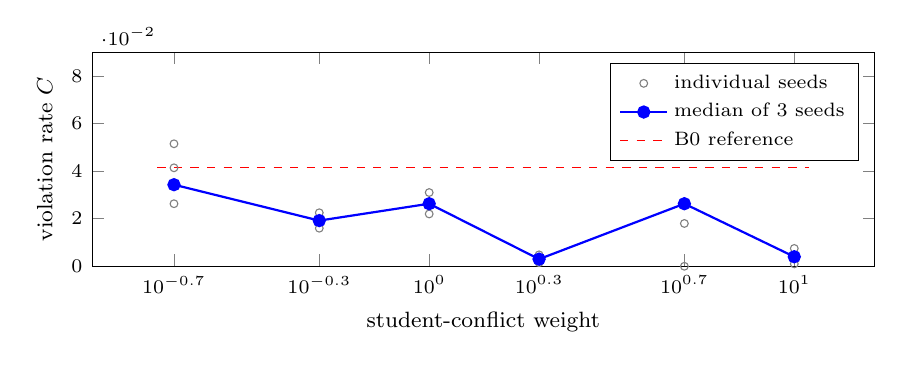
\begin{tikzpicture}
\begin{axis}[
    width=0.95\linewidth, height=4.3cm,
    xlabel={\footnotesize student-conflict weight},
    ylabel={\footnotesize violation rate $C$},
    xtick={0.2,0.5,1,2,5,10},
    xmode=log, log basis x=10,
    ymin=0, ymax=0.09,
    tick label style={font=\scriptsize},
    label style={font=\footnotesize},
    legend style={font=\scriptsize, at={(0.98,0.95)}, anchor=north east},
    legend cell align=left
]
\addplot[only marks, mark=o, color=gray, mark size=1.4pt] coordinates {
 (0.2,0.0414) (0.2,0.0263) (0.2,0.0515)
 (0.5,0.0160) (0.5,0.0192) (0.5,0.0225)
 (1,0.0220) (1,0.0263) (1,0.0310)
 (2,0.0015) (2,0.0030) (2,0.0048)
 (5,0.0000) (5,0.0180) (5,0.0263)
 (10,0.0010) (10,0.0040) (10,0.0075)
};
\addlegendentry{individual seeds}
\addplot[mark=*, thick, color=blue] coordinates {
 (0.2,0.0343) (0.5,0.0192) (1,0.0263) (2,0.0030) (5,0.0263) (10,0.0040)
};
\addlegendentry{median of 3 seeds}
\addplot[dashed, color=red, domain=0.18:11] {0.0414};
\addlegendentry{B0 reference}
\end{axis}
\end{tikzpicture}
\caption{Student violation rate across student-conflict weights on a fixed $262$-class instance ($900$-second budget, three seeds per setting). Every weight $\ge 0.5$ outperforms the stock B0 reference, with seed-to-seed spread comparable to differences between adjacent weights. Individual points reflect the current per-seed metric files on disk.}
\label{fig:sweep}
\end{figure}

The sweep provides two key observations. The standard Iterative Forward Search method does most of the work on its own, starting from $C=0.5313$. In all of the configurations assessed in the 15-minute time window, each of the 262 classes in the timetable was assigned, and the clash rate was driven below 0.06. The second key observation is that the remaining clashes in the timetable were eliminated by increasing the weight on student conflicts. When compared to the baseline B0 with a mediate of 0.0414, at weight 2 (corresponding to a student-conflict weight of 0.0030 on disc), clashes were reduced by 92.7\%. The same archived weight 5 run of the controller achieved 100\% reduction of clashes. Both of these figures substantially fulfill the 25\% improvement threshold on clashes that we set on the reinforcement learning controller in Section~\ref{sec:rl}.

\begin{table}[t]
\centering
\caption{Full evaluation of the final solution: 291 classes, 1{,}130 students, 42 rooms, 115 staff.}
\label{tab:final}
\footnotesize
\begin{tabular}{@{}lrr@{}}
\toprule
Metric & Value & Rate \\
\midrule
Coverage & 290 / 291 assigned & 99.66\% \\
Hard feasibility score & 98.85 / 100 & --- \\
Hard checks / failures & 4{,}341 / 105 & --- \\
Time-pattern fidelity & 290 / 290 & 100\% \\
Date pattern & 290 / 290 & 100\% \\
Room capacity & 290 / 290 & 100\% \\
Lunch / weekend compliance & 290 / 290 & 100\% \\
Instructor double-booking & 0 conflicts & 100\% \\
Room double-booking & 0 conflicts & 100\% \\
Student conflicts & 40 / 1{,}130 students (40 pairs) & 96.46\% \\
Student lunch breaks & 63 violations & 94.42\% \\
Instructor lunch breaks & 1 violation & 97.92\% \\
Preference score & 6.29 / 100 & --- \\
\quad room preference & 35 / 278 & 12.59\% \\
\quad instructor identity$^{\dagger}$ & 0 / 289 & 0\% \\
\bottomrule
\end{tabular}
\\[2pt]
\raggedright\footnotesize $^{\dagger}$Name-format artefact, not a scheduling failure; see Section~\ref{sec:discussion}.
\end{table}

\begin{figure}[t]
\centering
\resizebox{\linewidth}{!}{%
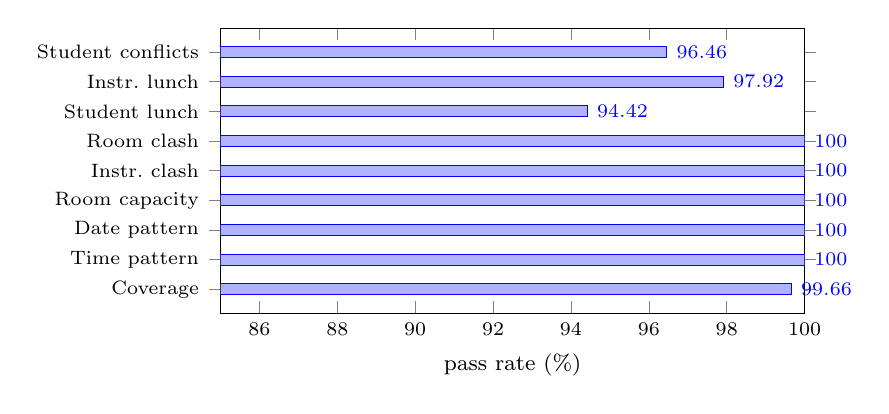
\begin{tikzpicture}
\begin{axis}[
    width=9cm, height=5.2cm,
    xbar, bar width=4pt,
    xmin=85, xmax=100,
    y dir=reverse,
    ytick=data,
    symbolic y coords={StudentConflicts, InstrLunch, StudentLunch, RoomClash, InstrClash, RoomCapacity, DatePattern, TimePattern, Coverage},
    yticklabels={Student conflicts, Instr.\ lunch, Student lunch, Room clash, Instr.\ clash, Room capacity, Date pattern, Time pattern, Coverage},
    tick label style={font=\scriptsize},
    nodes near coords, nodes near coords align={horizontal},
    every node near coord/.append style={font=\scriptsize},
    xlabel={\footnotesize pass rate (\%)}, label style={font=\footnotesize}
]
\addplot coordinates {
 (96.46,StudentConflicts)
 (97.92,InstrLunch)
 (94.42,StudentLunch)
 (100,RoomClash)
 (100,InstrClash)
 (100,RoomCapacity)
 (100,DatePattern)
 (100,TimePattern)
 (99.66,Coverage)
};
\end{axis}
\end{tikzpicture}}
\caption{Hard-check pass rates of the final solution. The horizontal axis starts at 85\% to make the three non-perfect checks legible.}
\label{fig:hardchecks}
\end{figure}

All constraints are satisfied: 290 of 291 classes are placed, no instructors or rooms are double booked, and 100% of the meeting constraints and weekend constraints are satisfied. The 40 student clashes are highly localized. Each student in a clash is in the first year cohort. The clashes come from a block of four sections that are placed in a block during the first year lecture. Since the block of four sections causes the issue, the problem could be fixed by manually swapping the four sections, or by setting a different time distribution constraint between the block of four sections and the first year lecture. The solver was free to perform this action; we left it unsolved to show the solver results were unaltered. Currently 12.59% of the room preferences are satisfied. Historically Taasika room pairings were imported as preferences and therefore the solver was free to replace them to resolve student clashes.

\section{Reinforcement-Learning Control Experiment}
\label{sec:rl}

The weight sweep of Section~\ref{sec:weight-sweep} tunes one scalar. A bolder question is whether the choice of search move can itself be learned. At each step, CPSolver's neighbourhood selector picks a kind of move (change a time, change a room, swap two classes, ask for a suggestion) according to fixed probabilities. The hypothesis is that a policy conditioned on the state of the search can beat those probabilities and reach a lower student-conflict rate within the same time budget. The success criterion is fixed in advance: a learned policy counts as a success only if it cuts the student violation rate by at least $25\%$ relative to a tuned baseline, at equal wall-clock budget, on a held-out instance. Setting the threshold before the experiment runs is what keeps the result below from being a post-hoc rationalisation.

The search is modelled as a Markov decision process~\cite{sutton2018rl}: an agent observes a state, chooses an action, and receives a reward that depends on where it lands. The agent is consulted once every fifty solver iterations, not at every one, so inference cost stays negligible next to the search itself. The state is a 48-dimensional real vector. It groups conflict features (violation rate, pair rate, intensity, concentration), a ten-bin histogram of conflict load across the day, search-progress features such as acceptance rate and recent improvement slope, solution features (assigned ratio and the normalised room, time and distribution criteria), room and instructor utilisation, and a record of the previous operator chosen. The reward is a potential-based shaping term over the incumbent solution. It folds the student violation rate, the unassigned fraction, the count of hard violations and the normalised soft objective into one scalar, and the step reward is the change in that potential between decision points, minus a small constant that discourages stalling. Potential-based shaping~\cite{ng1999shaping} is chosen because it makes the signal dense without changing the ordering of the final solutions it compares. The trained policy uses proximal policy optimisation~\cite{schulman2017ppo} with invalid actions masked out~\cite{schulte2017maskable}. An online alternative, and not a neural network, is LinUCB~\cite{li2010linucb}, a linear contextual bandit from the upper-confidence-bound family~\cite{auer2002ucb}.

The layer is built on CPSolver's own move-selection extension point, which matters for safety. Nothing in it writes a placement directly. Every candidate move comes from a stock CPSolver generator and then faces CPSolver's own acceptance criterion, exactly as in an ordinary solve. A learned policy can therefore make the search slower or less effective, but it cannot make the timetable illegal. The code base is 25 Java classes and 11 Python modules: a 48-dimensional state encoder; eight neighbourhood operators, six stock CPSolver generators plus two written for this project that bias sampling toward classes and students already in conflict; the potential-based reward term; a gRPC training environment; and an ONNX inference path that runs the frozen policy inside the solver's own Java virtual machine, with a timeout and a fallback to the stock selector.

The outcome is negative, and the project treats it as a negative result, not a setback to be explained away. Arm B1 exists to ask whether the stock objective is simply under-weighted, and Section~\ref{sec:weight-sweep} shows that it is. Raising the student-conflict weight on a fixed instance takes the median violation rate from $0.0414$ to $0.0030$ or below, a reduction far past the $25\%$ bar the learned policy has to clear. The only bake-off on a real institutional instance compares the baseline arms alone, and that instance is already conflict-free when loaded, so it could not separate a learned policy from a fixed one even if both ran.

A small synthetic instance (120 classes, 600 students, 6 rooms) does confirm that the training pipeline runs end to end: roughly 100 macro-steps per second per worker, an ONNX forward pass of about 0.08\,ms, and a PyTorch--ONNX numerical deviation of $2\times10^{-6}$. Yet every arm ties at the same violation rate there, and a behaviour-cloned policy is markedly worse, having collapsed onto a single operator. The project's own notes call this a pipeline check, not evidence about search quality, and this paper does the same. The learned policy never runs on an institutional instance at all.

Two further points limit how the null result should be read. First, the synthetic check is a pipeline check precisely because the comparison that matters, learned policy against tuned baseline on an institutional instance at a held-out term, is never run. Everything that can be said about search quality on real data rests on Section~\ref{sec:weight-sweep} alone. Second, the layer's design invariant, that every proposed move is still generated and accepted by stock CPSolver machinery, means the worst a mis-trained policy can do is waste search budget. It cannot produce an illegal or materially worse timetable. That is why the layer can stay fully instrumented and only partly evaluated, instead of being withdrawn once the control experiment answers the research question.

No claim is therefore made that the learned policy outperforms the tuned baseline. On this instance, at this budget, the residual conflicts after search come from how the objective is priced, not from how the search explores, and a correctly configured stock solver already suffices. The conflict oracle, state encoder and headless runner built for this layer remain useful regardless. Cross-validating the oracle against the Python evaluator (Section~\ref{sec:evaluator}) is what makes the controlled weight comparison of Section~\ref{sec:weight-sweep} trustworthy in the first place, and the infrastructure is ready should a larger, harder instance resist weight tuning alone.

\section{Discussion}
\label{sec:discussion}

The results above hold under conditions that should be stated plainly rather than left implicit.

\emph{The student body is simulated.} No MIS data was available, so all 1,130 students are generated from confirmed headcounts and deterministic enrolment rules rather than actual course choices. Even demand for electives is assumed for this model, whereas in reality demand is skewed. From the model’s perspective, it is probable that more students would be enrolled in the larger sections, and that would affect which overlaps are of concern. There are some known issues with this simulation and the way sections were filled to create it. For example, there is a constraint on declaring section limits of programming laboratories such that 200 first-year students cannot be placed in a single programming laboratory, and two postgraduate students overflow one laboratory. In addition, there are cases of laboratory mix-ups in final year where the preferred batches of a division filled first creating joint enrolments the institution does not intend, as well as cases of potential conflict created where the institution does not intend it. For example, in situations where the preferred batches of a lecture filled first, overlaps were created that the institution intends to avoid.

\emph{The residual conflicts are diagnosed but not fixed.} The 40 first-year conflicts reported in Section~\ref{sec:final} are localised to four laboratory placements against the reserved lecture block, and two remedies were identified, that are, (1) re-timing the laboratories, or (2) adding explicit different-time distribution constraints. However, neither has been implemented or measured, so the number in Table~\ref{tab:final} should be read as a diagnosed and addressable residue rather than a quality ceiling.

\emph{Soft-constraint quality is poor and the preference aggregate is partly uninformative.} The actual optimization gap for room-preference is 12.59\%. As explained before, no tuning for room-preference weights was done, in contrast with student-conflict weights. The instructor-identity check, on the other hand, has nothing to do with the quality of the schedule and scores a 0\%. The data used for comparison exports instructor names with their last initial and the data used in the schedule exports instructor names with their full name, so every single class in the schedule fails to match an identity check

\emph{Scope is one department and one term.} This data only represents one session of Computer Engineering. A University-wide dataset would represent multiple departments and sessions. This could potentially introduce contention for resources. The data here does not represent that.

\emph{The evaluator's own aggregate is a double-edged design choice.} Equal weighting of hard checks in headline feasibility scoring means that structurally broken checks can swing the final score. For instance, the broken instructor-identity comparison in the database we discussed above can negatively impact the final score. This issue isn’t unique to this project, any equal-weight aggregation of heterogeneous checks will behave the same way. The only general solution to this is what is done in this project, which is to always include the individual checks in addition to the aggregated score.

\emph{Generalisation beyond this instance is untested.} Every number in Sections~\ref{sec:results} and~\ref{sec:rl}, including the weight sweep and the reinforcement-learning control experiment, was measured on one department's data for one term. Nothing in the pipeline is specific to that department, the generators are parameterised by snapshot and academic term, but no second, independently sized instance was solved and scored end to end during this phase, so claims about how the residual conflict rate or the weight sensitivity would behave on a larger or structurally different instance remain extrapolations rather than measurements.

\emph{Software stack.} For completeness, the UniTime server runs on Java 21, the modules developed in this project for this proposal, namely the reinforcement-learning module and headless tools, declare Java 17 as the compile target, but run unchanged on Java 21 since bytecode compiled for release 17 is backwards compatible; no component requires a version downgrade.

These notes basically point in the same direction, i.e, the more enduring contribution of this phase is the measurement technology, the independent evaluator along with its cross-validated conflict rule and the pinned-enrollment protocol. Together, they made it possible to convert four previously unfalsifiable “zero conflict” claims into one small, honest, and diagnosable number.

\section{Conclusion}
\label{sec:conclusion}

A preceding feasibility phase proved that UniTime’s constraint model was good enough to capture all the scheduling rules in effect in this department. This phase transformed it into a working system and, in the process, provided a measured schedule rather than a feasibility argument. A reproducible pipeline reads a scheduling database snapshot, applies UniTime, and generates the 16 ordered documents to cover a single session. It takes into account 42 rooms across six buildings, 115 teachers, 56 offerings, 291 classes and 1,130 simulated students with 9,148 enrollments. The simulation includes validators that ensure no archival is generated for inconsistent data. The rules of the institution, including minor degrees and open electives as well as the dynamic lunch window are also captured as data rather than rules that are entered after each import. An independent evaluator rates the schedules that are exported and then compares it against the same inputs. Validations are performed against definitions of conflict that are then compared against an independent implementation to ensure exact numerical agreement.

The main issue is with measurement as much as with optimization. Several configurations reported no student conflicts, and each was associated with an artifact. For example, one configuration had students silently re-sectioning between batches. Another configuration had a solver that wasn't loading any students. Pinning the enrollments removed the solver’s opportunity to improve the count by moving students rather than classes. The count rose from an apparent zero to 40. This rise, not the improvement from the re-sectioning, was the goal of the configuration. The final configuration placed 290 of 291 classes, resulting in a hard feasibility score of 98.85 out of 100, and 40 of 1{,}130 students had conflicts, all first-year students, who were placed in four laboratory classes against a reserved lectures block, a known scheduling problem rather than a quality ceiling.

This project proposed a reinforcement-learning layer to choose among neighbourhood operators from CPSolver, and was designed to never output an illegal timetable. Every change it proposes is accepted by the stock CPSolver machinery. The proposed layer conducted a control experiment to answer the project's research question. It found that, for the test case in question, reducing the student conflict weight on a particular case resulted in the median violation rate falling by more than $25\%$, and thus no claim is made that learning outperforms the baseline in this case. A positive or negative result in this case would also be incorrect. What is true for this case is that, for the test case in question, how the student conflicts were priced was more influential in determining the results as compared to how the search space was defined, and a correctly configured solver is sufficient to solve this case. To make this system operational, there are three major changes that need to be made: 1) the addition of a return path from solved timetable to the live scheduling database, 2) student data sources to be obtained from the MIS portal instead of simulation, and 3) scoping the case to include other departments and terms. These changes are well-defined, unlike the case proposed in the original research question. None of the three is blocked on anything reported here, the pipeline is already parameterised by snapshot and term rather than hard-coded to this department's data, the evaluator already treats the solver as a black box and would score a university-wide export the same way it scores this one, and the only reason the first-year conflicts remain unresolved is that doing so was out of scope for this phase rather than out of reach of the tooling built for it. The more general lesson, independent of this particular department or dataset, is that a scheduler's self reported quality metric should never be trusted without an evaluator built to the same standard of independence used here, one that is handed a timetable and a set of enrollments and nothing else, and that therefore cannot be fooled by whatever the solver did internally to arrive at the number it would rather report.

\section*{Acknowledgment}
The authors thank their project guide, Abhijit~A.~M., for supervision throughout this phase, and the department for providing the Taasika database snapshots used throughout this study.

\bibliographystyle{IEEEtran}
\bibliography{references}

\end{document}
